%%% File encoding is UTF8

%%% If you use this template then please give credit like this:
%%% ----------------------------
% LaTeX code inspired by the LaTeX Thesis Template by Manuel Kuehner 
% www.bedienhaptik.de/latex-template/
%%% ----------------------------

% ##############################################
% Start: Template Preamble
% ##############################################
%

% Documentclass definition
%%% File encoding is UTF8
%%% You can use special characters just like ä,ü and ñ

% KOMA-Script class 'scrbook'
% Link to the documentation: 
% German: http://mirrors.ctan.org/macros/latex/contrib/koma-script/doc/scrguide.pdf
% English: http://mirrors.ctan.org/macros/latex/contrib/koma-script/doc/scrguien.pdf
% CTAN: http://www.ctan.org/pkg/koma-script
% Author of the KOMA-Script family is Markus Kohm
\documentclass[paper=letter % Letter is "carta"
			 , fontsize=10pt % Arial 10 for all text.
			 , headings=big
			 , parskip=half-
			%, noparskip % No par skip. If yes park skip the command is parskip
			%, numbers=noendperiod % 2.3.1 vs 2.3.1. (no dot after the last chapter number)
			 , numbers=endperiod
	         , twoside=false
			% , toc=bibliography % Bibliography appears in Table of Contents (without a number)
			% , toc=listof % List of Figures and List of Tables appear in Table of Contents
			% , chapterprefix=true
			 , chapterprefix=false
			% , bibliography=totoc % The bibliography will have an entry at the table of contents but no number.
			 , numbers=noenddot
			 , titlepage=simple
			 , headings=onelinechapter
			 , version=last % Use latest version of the KOMA-Script
			 , final
]{scrbook}

\RedeclareSectionCommand[
afterskip=\parskip]{chapter}
\RedeclareSectionCommand[
beforeskip=\parskip
, afterskip=0.1\parskip]{section}
\RedeclareSectionCommand[
beforeskip=1.1\parskip plus 3mm
, afterskip=0.1\parskip]{subsection}


\KOMAoption{bibliography}{leveldown}

\newcommand{\mychapter}[1]{%
	\chapter{#1}
	\addcontentsline{lof}{chapter}{%
		Figuras del Capítulo \thechapter: #1 \vspace{10pt}
	}
}

\addtokomafont{section}{\large}
\addtokomafont{subsection}{\normalsize}  %1.1.1 Minus size: 10 % normalsize is 10

%REVISAR
\usepackage[compact]{titlesec}

% Titles in the chapters, not in TOC.
\titleformat{\chapter}
{\bfseries\Large\vspace*{-4.0cm}}	% Formato título
{	% Contenido de la etiqueta
	\filright
	\Large\MakeUppercase\chaptertitlename\ \thechapter.\ 
}
{0pt} % Espacio mínimo entre etiqueta y cuerpo
{\filright\MakeUppercase} % Código que precede al cuerpo del título
[\vspace{1.5pt}] % Margen de 1.5pt

\titleformat{\section}
{\bfseries\large\vspace{2pt}}
{\large\MakeUppercase\thesection\ \vspace{2pt} } % 3 espacios luego del titulo de una seccion
{0pt}
{\MakeUppercase}
[\vspace*{0.5cm}]

\titleformat{\subsection}
{\bfseries\normalsize\vspace{2pt}} % 3 espacios luego del titulo de una seccion
{\normalsize\thesubsection\ }
{0pt}
{\vspace*{0.5cm}}

\titleformat{\subsubsection}
{\itshape\normalsize\vspace{1.0cm}}
{\itshape\thesubsubsection\ }
{0pt}
{\vspace*{0.5cm}\itshape}

\titlespacing*{\chapter} {0pt}{85pt}{20pt} 
\titlespacing*{\section} {0pt}{6.5ex plus 1ex minus .2ex}{2.3ex plus .2ex}
\titlespacing*{\subsection} {0pt}{6.5ex plus 1ex minus .2ex}{2.3ex plus .2ex}
\titlespacing*{\subsubsection}{0pt}{3.25ex plus 1ex minus .2ex}{1.5ex plus .2ex}
\titlespacing*{\paragraph} {0pt}{3.25ex plus 1ex minus .2ex}{1em}
\titlespacing*{\subparagraph} {\parindent}{3.25ex plus 1ex minus .2ex}{1em}


% Loading additional packages from the KOMA-Script family
%%% File encoding is UTF8
%%% You can use special characters just like ä,ü and ñ

% Special KOMA-Script package - I added it because I also use the float package in this template, see: 
% http://tex.stackexchange.com/questions/51867/koma-warning-about-toc
% CTAN: http://www.ctan.org/tex-archive/macros/latex/contrib/koma-script/doc
\usepackage{scrhack}

% Better support for marginnotes
% new command: \marginnote
% LaTeX standard command: \marginpar
% CTAN: http://www.ctan.org/pkg/marginnote
\usepackage{marginnote}

% Extended header and footer support
% CTAN: http://www.ctan.org/pkg/scrpage2
\usepackage[automark
  		  , ilines
		  , headsepline
		  , footsepline
]{scrpage2}

\usepackage{setspace}
\onehalfspace

% Page layout definition
%%% File encoding is UTF8
%%% You can use special characters just like ä,ü and ñ

% User friendly interface to change layout parameters
% CTAN: http://www.ctan.org/pkg/geometry
\usepackage{geometry}
\geometry{%
	%bottom=30mm,
	, showframe=false % For debugging: try true and see the layout frames
	%, margin=30mm
	%, marginparsep=3mm
	%, marginparwidth=20mm
	, headheight=14pt
	, top=2.5cm
	, bottom=2.5cm 
	, left=4cm
	, right=2.5cm
	, letterpaper
}



% Standard packages
%%% File encoding is UTF8
%%% You can use special characters just like ä,ü and ñ

% Input encoding is 'latin1' (Latin 1 - also known as ISO-8859-1)
% CTAN: http://www.ctan.org/pkg/inputenc
% 
% A newer package is available - you may look into:
% \usepackage[x-iso-8859-1]{inputenc}
% CTAN: http://www.ctan.org/pkg/inputenx
%\usepackage[latin1]{inputenc}
\usepackage[utf8]{inputenc}

% Font Encoding is 'T1' -- important for special characters such as Umlaute ü or ä and special characters like ñ (enje)
% CTAN: http://www.ctan.org/pkg/fontenc
\usepackage[T1]{fontenc}

% Language support for 'english' (alternative 'ngerman' or 'french' for example)
% This case is in spanish
% CTAN: http://www.ctan.org/pkg/babel
%\usepackage[english]{babel} 
\usepackage[spanish
          , es-tabla
          , es-noindentfirst]{babel} 

% Doing calculations with LaTeX units -- needed for the vertical line in the footer
% CTAN: http://www.ctan.org/pkg/calc
\usepackage{calc}

% Extended graphics support 
% There is also a package named 'graphics' - watch out!
% CTAN: http://www.ctan.org/pkg/graphicx
\usepackage{graphicx}

% Extendes support for floating objects (tables, figures), adds the [H] placing option (\begin{figure}[H]) which palces it "Here" (without any doubt).
% CTAN: http://www.ctan.org/pkg/float
\usepackage{float}

% Extended color support
% I use the command \definecolor for example. 
% Option 'Table': Load the colortbl package, in order to use the tools for coloring rows, columns, and cells within tables.
% CTAN: http://www.ctan.org/pkg/xcolor
\usepackage[table]{xcolor} 

% Nice tables
% CTAN: http://www.ctan.org/pkg/booktabs
\usepackage{booktabs}

\usepackage{colortbl}

\usepackage{multirow,siunitx}

% Better support for ragged left and right. Provides the commands \RaggedRight and \RaggedLeft. 
% Standard LaTeX commands are \raggedright and \raggedleft
% http://www.ctan.org/pkg/ragged2e
\usepackage{ragged2e}

% Create function plots directly in LaTeX
% CTAN: http://www.ctan.org/pkg/pgfplots
\usepackage{pgfplots}
\pgfplotsset{compat=1.11}

% Main Font used: Arial
\usepackage{uarial}
\usepackage[expert]{mathdesign}
\renewcommand{\familydefault}{\sfdefault}

% tocloft ? Control table of contents, figures, etc
% CTAN: https://ctan.org/pkg/tocloft
%\usepackage{tocloft}

% Configure Microtype
\usepackage[activate={true,nocompatibility},final,tracking=true,kerning=true,spacing=true,factor=1100,stretch=10,shrink=10]{microtype}
% activate={true,nocompatibility} - activate protrusion and expansion
% final - enable microtype; use "draft" to disable
% tracking=true, kerning=true, spacing=true - activate these techniques
% factor=1100 - add 10% to the protrusion amount (default is 1000)
% stretch=10, shrink=10 - reduce stretchability/shrinkability (default is 20/20)

\SetExtraKerning[unit=space]
{encoding={*}, family={bch}, series={*}, size={footnotesize,small,normalsize}}
{\textendash={400,400}, % en-dash, add more space around it
	"28={ ,150}, % left bracket, add space from right
	"29={150, }, % right bracket, add space from left
	\textquotedblleft={ ,150}, % left quotation mark, space from right
	\textquotedblright={150, }} % right quotation mark, space from left

\SetExtraKerning[unit=space]
{encoding={*}, family={qhv}, series={b}, size={large,Large}}
{1={-200,-200}, 
	\textendash={400,400}}

% Use French spacing
\frenchspacing



% https://www.ctan.org/pkg/biblatex-ieee
\usepackage[backend=biber
		  %, style=ieee % Esta bien, pero no agrupa las citaciones
		  %, style=numeric-comp %Revisar, porque algunas referencias no las tira correctas
		  %Antes: IEEE
		  %, bibstyle=ieee  %Combinacion de ambas
		  %, citestyle=numeric-comp
		  %AHORA: APA
		  , style=apa
		  , hyperref=true
		  , url=false
		  , isbn=false
		  , backref=true
		 %, style=custom-numeric-comp
		  , citereset=chapter
		  , maxcitenames=3
		  , maxbibnames=100
		  , block=none
		  %, sorting=none % El orden de las citas en IEEE es según el orden de aparicion en el texto
		  , sortcites=true
		  , sorting=nyt
		  % APA no tiene referencias cruzadas, si se quiere desactivar, comentar apabackref
		  , apabackref=true
		  , language=spanish
]{biblatex}
\bibliography{bibfile}

% Separacion entre entradas de la referencia
\setlength\bibitemsep{\baselineskip}

\DeclareLanguageMapping{spanish}{spanish-apa}

\usepackage[style=english]{csquotes}

%TODO: Cambiar de bibliografia a Referencias Bibliograficas
\renewcommand\bibname{Referencias Bibliogr\'aficas}
\DefineBibliographyStrings{spanish}{%
	andothers = {\em et\addabbrvspace al\adddot}
}

\AtEveryBibitem{%
	\ifboolexpr{test {\ifentrytype{article}} and not test {\iffieldundef{doi}}}
	{\clearfield{number}}
	{}%
}

\usepackage{pgfplotstable}

%FIX: dont work
\usepackage[noabbrev,capitalize,nameinlink,spanish]{cleveref}
\crefname{table}{\spanishtablename}{\spanishtablename}

\usepackage{subcaption}

\usepackage{neuralnetwork}

\usepackage[linesnumbered
		   , algoruled
	       , vlined
	       , boxed
	       , algochapter
	       , commentsnumbered
	       , spanish
	       , onelanguage
]{algorithm2e}

\usepackage{pgfgantt}
\ganttset{
	, y unit title=0.5cm
	, y unit chart=0.7cm
	, vgrid,hgrid
	, progress=today
	, group/.append style={orange}
	, milestone/.append style={red}
	, progress label node anchor/.append style={text=red}
	, bar/.style={draw=black, fill=gray!50}
	, incomplete/.style={draw=black, fill=white}
	, title height=1
	, title label font=\bfseries\footnotesize
	, bar/.style={fill=black}
	, bar height=0.7
	, today label=HOY
	, group right shift=0
	, group top shift=0.7
	, group height=.3
	, group peaks width={0.2}
	, inline
} 

\usepackage{graphicx}
\usepackage{xcolor}

\usepackage{amsmath,amssymb}


% Use Spanish file for hyphenation
\hyphenation{hyph-es}

% ####-Important-####
%
% Definition of the two main colors
% -----------------------
% The corresponding xcolor package ist loaded in the file 
% 01_Preamble/StandardPackages.tex
%
% ####-Important-####
\definecolor[named]{myColorMainA}{RGB}{0,0,0}
\definecolor[named]{myColorMainB}{RGB}{0,0,0}
\definecolor{mylinkcolor}{RGB}{5,123,10}
\definecolor{mycitecolor}{RGB}{5,10,123}

% colors
\definecolor{gray75}{gray}{0.75}
\definecolor{gray90}{gray}{0.90}
\definecolor{darkblue}{rgb}{0,0,0.5}
\definecolor{darkgreen}{rgb}{0,0.5,0}
\definecolor{green}{rgb}{0.2,0.8,0.2}
\definecolor{red}{rgb}{1.0,0.3,0.0}
\definecolor{orange}{rgb}{1.0,0.6,0.0}

% Customization of 
% - Floating Objects (Caption) 
% - Table of Contents (TOC)
% - List of Figures
% - List of Tables
% - Headings (like chapter, section, etc.)
% - Bibliography Style
%%% File encoding is UTF8
%%% You can use special characters just like ä,ü and ñ

% ##############################################
% Start: Table of Contents (TOC) Customization
% ##############################################
%

% Level for numbered captions
\setcounter{secnumdepth}{5}

% Level of chapters that appear in Table of Contents
\setcounter{tocdepth}{5} % bis wohin ins Inhaltsverzeichnis aufnehmen
% -2 no caption at all
% -1 part
% 0  chapter
% 1  section    
% 2  subsection 
% 3  subsubsection
% 4  paragraph
% 5  subparagraph

% KOMA-Script code to adjust TOC
% Applying the color 'myColorMainA' which is defined in the main file (MainFile.tex)
\makeatletter
%Dont use color
\addtokomafont{chapterentrypagenumber}{\color{myColorMainA}}
\addtokomafont{chapterentry}{\color{myColorMainA}}
\makeatother

\renewcaptionname{spanish}{\contentsname}{\hfill\bfseries\Large Tabla de Contenidos \hfill} % Table of contents in spanish
\renewcaptionname{spanish}{\listfigurename}{\hfill\bfseries\Large \'Indice de Figuras \hfill}    %Figures
\renewcaptionname{spanish}{\listtablename}{\hfill\bfseries\Large \'Indice de Tablas \hfill}        %Tables

%Funciona
\makeatletter
\let\oldaddchaptertocentry\addchaptertocentry
\renewcommand{\addchaptertocentry}[2]{%
	\oldaddchaptertocentry{}{\@chapapp{} #1. #2}}
\let\oldaddparttocentry\addparttocentry
\renewcommand{\addparttocentry}[2]{%
	\oldaddchaptertocentry{}{\partname{} #1. #2}}

\RedeclareSectionCommand[tocindent=5.5em]{section}
\RedeclareSectionCommand[tocindent=7.8em]{subsection}

\makeatother

\makeatletter
\newcommand{\chapterwithfigures}{\addxcontentsline{lof}{chapteratlist}[{\thechapter}]{\scr@ds@tocentry}}%
\makeatother

%
% #######################
% End: Table of Contents (TOC) Customization
% #######################

% ##############################################
% Start: Floating Object Customization
% ##############################################
%

% Extended support for catioons of figures and tables etc.
% CTAN: http://www.ctan.org/pkg/caption
\usepackage[font={small}
		  %, labelfont={bf,sf}
		  , labelfont={sf}
		  , format=hang % try plain or hang
		  , margin=5pt
]{caption}
%

\newcommand{\englishword}[1]{\textit{#1}}

\newcommand{\ingles}[1]{\textit{#1}}
\newcommand{\producto}[1]{\textit{#1}}
\newcommand{\tecnologia}[1]{\textit{#1}}

\newcommand*{\captionsource}[2]{%
	\caption[{#1}]{#1}
	\par\centering\small{Fuente: #2.}
}

\newcommand*{\captiontable}[2]{%
	\captionabove[{#1}]{#1 \par\centering \small{Fuente: #2.}}
}

% Make Uppecase section title
\addtokomafont{section}{\MakeUppercase}

% Tables with PGFPlots
\usepackage{pgfplotstable} % Generates table from .csv
\usepgfplotslibrary{colorbrewer}
\usepgfplotslibrary{statistics}

\pgfplotsset{cycle list/Dark2}
\pgfplotsset{cycle list/Dark2-5}

% Table: htb: place here, top, or bottom, BUT NEVER at other page
%Args: 
% 1: Caption
% 2: Source
% 3: CSV File (separated by semicolons ;)
% 4: Label command
\newcommand{\insertTableFile}[4]{
	\begin{table}[htb]
	\centering
	\captiontable{#1}{#2}
	\pgfplotstabletypeset[
	every even row/.style={
		before row={\rowcolor[gray]{0.9}}},
	every head row/.style={
		before row=\toprule,after row=\midrule},
	every last row/.style={
		after row=\bottomrule},
	col sep=semicolon, 
	string type]{#3}
	#4 % Label command		
	\end{table}
}


% Arg 1: X label
% Arg 2: Y label
% Arg 3: Filename
% Arg 4: Caption
% Arg 5: Source
% Arg 6: Label

\newcommand{\plotFile}[3]{
	\pgfplotsset{cycle list/Dark2}
	\begin{figure}[htb]
	\centering
	\begin{tikzpicture}
	\begin{axis}[
	xlabel={#1},
	ylabel={#2},
	xmin=0,
	ymin=0,
	ymax=1,
	legend style = {
		legend pos = outer north east,
	},
	%cycle list name=Dark2,
	width=0.7\textwidth
	]
	\legend{Legend 1}
	\pgfplotstableread{#3}\leg1;
	\addplot+ [
	cycle list name=Dark2,
	mark=square*
	] table []{\leg1};
	\end{axis}
	\end{tikzpicture}
	%\captionsource{#4}{#5}
	%#6	
	\end{figure}

}

\newcommand{\correcion}[1]{\hl{#1}}
\newcommand{\currentYear}{2017}
\newcommand{\fuentePropia}{Elaboración propia, (\currentYear)}


%% References
\newcommand{\tab}[1]{Tabla~\ref{#1}}
\newcommand{\tabla}[1]{Tabla~\ref{#1}}
\newcommand{\fig}[1]{Figura~\ref{#1}}
\newcommand{\alg}[1]{Algoritmo~\ref{#1}}
\newcommand{\eq}[1]{Ecuación~\ref{#1}}


% #######################
% End: Floating Object Customization
% #######################

% ##############################################
% Start: Headings Customization
% ##############################################
%

% KOMA-Script code to customize the headings
% Applying the color 'myColorMainA' which is defined in the main file (MainFile.tex)
%\addtokomafont{chapter}{\color{myColorMainA}}
%\addtokomafont{section}{\color{myColorMainA}}
%\addtokomafont{subsection}{\color{myColorMainA}}
%\addtokomafont{subsubsection}{\color{myColorMainA}}
%\addtokomafont{paragraph}{\color{myColorMainA}}
%\addtokomafont{subparagraph}{\color{myColorMainA}}

% #######################
% End: Headings Customization
% #######################


% Customization of the header, footer and teh margin note
%%% File encoding is UTF8
%%% You can use special characters just like ä,ü and ñ

% Custom command fpr the margin notes: \myMarginnote{Your Text}
% Comment on the \lineskiplimit=-\maxdimen:
% See http://tex.stackexchange.com/questions/49072/
% Without it the line spacing of the normal text was changed (ugly).
\newcommand{\myMarginnote}[1]{%
	\marginnote{% needs marginnote package
		\ifthispageodd{\RaggedRight}{\RaggedLeft}% needs ragged2e package
		\color{myColorMainB}%
		\lineskiplimit=-\maxdimen% 
		\normalfont\sffamily\scriptsize%
		#1}%
}

% ##############################################
% Start: Header and Footer Customization
% ##############################################
%



% KOMA-Script code for header and footer font
\setkomafont{pageheadfoot}{%
	\normalfont\sffamily\bfseries
	}
\setkomafont{pagefoot}{%
	\normalfont\sffamily
	}
\setkomafont{pagenumber}{%
	\normalfont\rmfamily
	}

% Define width of header
%\setheadwidth[0pt]{textwithmarginpar}

% Define with of header line
\setheadsepline{0.4pt}

% Define width of footer
\setfootwidth[0pt]{text}
% Define with of footer line (here: no line)
\setfootsepline[text]{0pt}

% Some calculations
% calc package is needed which is loaded here: 01_Preamble/CommonPackages.tex
% If you want to understand the calculations visit:
% http://en.wikibooks.org/wiki/LaTeX/Page_Layout
\newlength{\myLenghthFootAbstand}
\setlength{\myLenghthFootAbstand}{\paperheight-1in-\topmargin- \headheight-\headsep-\textheight-\footskip}
\newlength{\myLenghthTemp}
\setlength{\myLenghthTemp}{\myLenghthFootAbstand+\baselineskip}

% Define content of header and footer
% Using some scrpage2 commands here. The scrpage2 package is loaded here: 01_Preamble/KOMA-Script-Packages.tex
% Some LaTeX magic...
% Clear all defaults
\clearscrheadfoot
% Header
\ohead{\textcolor{myColorMainA}{\headmark}}

% Footers
\lefoot[\pagemark]{\pagemark}
\rofoot[\pagemark]{\pagemark}

\automark[section]{chapter}


%
% #######################
% End: Header and Footer Customization
% #######################

% Optimize paragraphs (avoid overfull... warnings)
%%% File encoding is UTF8
%%% You can use special characters just like ä,ü and ñ

% This is an suggestion from Axel Reichert (LaTeX package author)
% See CTAN: http://www.ctan.org/author/reichert
% See CTAN: http://www.ctan.org/pkg/l2tabu-english (Cgapter: 1.8 Should I use \sloppy?)

\tolerance 1414
\hbadness 1414
\emergencystretch 1.5em
\hfuzz 0.3pt
\widowpenalty=10000
\vfuzz \hfuzz
\raggedbottom

% Interlineado de 1.5:
\renewcommand{\baselinestretch}{1.5}

\setlength{\parindent}{1em}
%\setlength{\parindent}{4em}
\setlength{\parskip}{\baselineskip}
%\parskip = \baselineskip
%\setlength{\parskip}{0.3em}
%\parskip = 2\baselineskip % no shrink and no stretch

% PDF related packages
%%% File encoding is UTF8
%%% You can use special characters just like ä,ü and ñ

% Package for PDF features such as bookmarks and hyperlinks. 
% Important: Should be loaded at the end.
% CTAN: http://www.ctan.org/pkg/hyperref
\usepackage[bookmarks			   % Create bookmarks
		  , bookmarksopen=true,    % Unfold bookmatk tree in PDF viewer when document is opened
		  , bookmarksopenlevel=1   % Level of unfolding
		  , bookmarksnumbered=true % Number bookmarks
		  , hidelinks              % do not highlight hyperlinks -- looks ugly
		  , pdfpagelabels=true     % See manual...
		  , plainpages=false       % See manual...
		  , hyperfootnotes=true    % Hyperlinks for footnotes
		  , hyperindex=true        % Indexeinträage verweisen auf Text
		 % Links, solo en version PDF virtual
		  , colorlinks=true
		  , linkcolor=darkblue     % Color of internal links
		  , citecolor=darkblue     % Color of links to bibliography
		  , filecolor=darkblue     % Color of file links
		  , urlcolor=darkgreen     % Color of external links
		  , pdftex
		  , pdftitle={Modelo predictivo del desempeño de búsqueda de información en línea en estudiantes de educación básica}
		  , pdfauthor={Gonzalo Javier Martinez Ramirez}
		  , pdfsubject={Tesis de grado}
		  , pdfkeywords={Alfabetización informacional, competencias de investigación en línea, comportamiento de estudiantes, minería de datos, modelos de clasificación.}
		  , pdfcreator={pdflatex}
]{hyperref}

% PDF related packages
%%% File encoding is UTF8
%%% You can use special characters just like ä,ü and ñ

% Package to create test text -- just for demonstration purposes
% The command \blindtext produces a test text -- good for testing the layout
% CTAN: http://www.ctan.org/pkg/blindtext
\usepackage[]{blindtext}
% The custom command \myMarginnote is defined in the file: 
% 01_Preamble/HeaderFooterMarginnote.tex
\renewcommand{\blindmarkup}[1]{\myMarginnote{#1}}

% Bibliography
%%% File encoding is UTF8
%%% You can use special characters just like ä,ü and ñ

%% Bibliography style

% Prints author names as small caps
%\renewcommand{\mkbibnamefirst}[1]{\textsc{#1}}
%\renewcommand{\mkbibnamelast}[1]{\textsc{#1}}
%\renewcommand{\mkbibnameprefix}[1]{\textsc{#1}}
%\renewcommand{\mkbibnameaffix}[1]{\textsc{#1}}

% document preamble
% removes period at the very end of bibliographic record
%\renewcommand{\finentrypunct}{}

%\renewcommand{\newunitpunct}{\addspace\midsentence}

\DeclareUnicodeCharacter{00A0}{ }

\DefineBibliographyStrings{english}{%
	backrefpage  = {\lowercase{s}ee p.}, % for single page number
	backrefpages = {\lowercase{s}ee pp.} % for multiple page numbers
}

\DefineBibliographyStrings{spanish}{%
	backrefpage  = {\lowercase{v}er pág.}, % for single page number
	backrefpages = {\lowercase{v}er págs.} % for multiple page numbers
}


%\DeclareFieldFormat{journaltitle}{\mkbibemph{#1},} % italic journal title with comma
%\DeclareFieldFormat[inbook,thesis]{title}{\mkbibemph{#1}\addperiod} % italic title with period
%\DeclareFieldFormat[article]{title}{#1} % title of journal article is printed as normal text

% makes volume of journal bold and adds colon
%\DeclareFieldFormat[article]{volume}{\textbf{#1}\addcolon\space}

% removes pagination (p./pp.) before page numbers
%\DeclareFieldFormat{pages}{#1}

%%
% Footnote
%

% new command \sjcitep prints footnote citation above punctuation
\newlength{\spc} % declare a variable to save spacing value
\newcommand{\sjcitep}[2][]{% new command with two arguments: optional (#1) and mandatory (#2)
	\settowidth{\spc}{#1}% set value of \spc variable to the width of #1 argument
	\addtolength{\spc}{-1.8\spc}% subtract from \spc about two (1.8) of its values making its magnitude negative
	#1% print the optional argument
	\hspace*{\spc}% print an additional negative spacing stored in \spc after #1
	\supershortnotecite{#2}}% print (cite) the mandatory argument

%
% #######################
% Ende: Template Preamble
% #######################

% ##############################################
% Start: Document
% ##############################################
%
% ------------------------------------------------------------------
\begin{document}

% Title page
%%% File encoding is ISO-8859-1 (also known as Latin-1)
%%% You can use special characters just like ä,ü and ñ

% Title page using \maketitle (a more flexible alternative is the titlepage environment)
%\title{PHD Thesis}
%\subtitle{\LaTeX{} template by Manuel Kuehner\\ \url{www.bedienhaptik.de/latex-template/}}
%\author{Manuel Kuehner}
%\date{01.01.2015}


%\maketitle
\def\alumno#1{Gonzalo Martinez Ramirez}
\def\rut#1{18.045.598\ -\ 1}
\def\ingreso#1{2010}
\def\fono#1{(+56)\ 9\ -\ 96112973}
\def\mail#1{gonzalo.martinez@usach.cl}
\def\profesorguia#1{Roberto Ignacio González Ibañez}

\newgeometry{top=4cm, bottom=2.5cm, left=4cm, right=2.5cm}
\begin{titlepage}
	\begin{center}
		{\Large\bfseries UNIVERSIDAD DE SANTIAGO DE CHILE} \\ 
		{\large\bfseries FACULTAD DE INGENIERÍA} \\
		{\large\bfseries Departamento de Ingeniería Informática} \\

		\begin{picture}(18,4)(0,40)
		\put(160,50){
\includegraphics[width=0.15\textwidth]{03_GraphicFiles/logo-onlyescudo-usach-bw}}
		\end{picture}
		
		% ----------------------------------------------------------------
		%\vspace{5cm}
		\vspace*{\fill}
		{\Large\bfseries \MakeUppercase TITULO DE LA PROPUESTA/TESIS} \\ %[5pt]
		{\bfseries Propuesta de Tesis}
		\vspace*{\fill}
		% ----------------------------------------------------------------
	
		\vfill
		\begin{flushright}
			\begin{tabular}[t]{rl}
				Nombre: & Gonzalo Javier Martinez Ramirez \\
				R.U.T.: & 18.045.598-1 \\
				A\~no Ingreso: & 2010 \\
				Tel\'efono: & (+56) 9 96112973 \\
				E-mail: & gonzalo.martinez@usach.cl \\
				Profesor Patrocinador: & \profesorguia \\ 
			\end{tabular}
		\end{flushright}
	
		%\vspace{1cm}
		%\hspace{6.8cm}
		%\begin{tabular}{p{5.5cm}}
		%Trabajo de titulación presentado en conformidad a los requisitos para obtener el grado de Magister en Ingeniería Informática.
		%\end{tabular}
		\vfill
		{Santiago\ \textendash \ Chile} \\
		{Junio\ 2017}
	\end{center}
\end{titlepage}
\restoregeometry
% Empty page after title page
\cleardoublepage

% Activate header and footer defined in the file:
% 01_Preamble/HeaderFooterMarginnote.tex
\pagestyle{scrheadings}

% Activate roman numbering (e. g. xii)	
\pagenumbering{roman}

% Start with page 1 (I)
\setcounter{page}{1}

% Abstract
%%% File encoding is UTF8
%%% You can use special characters just like ä,ü and ñ

% Chapter without numbering but with appearance in the Table of Contents
% \addchap is a command from KOMA-Script
%\addchap*{Abstract}

\chapter*{\centerline{Resumen}} \vspace{-6em}
Durante la última década, debido a los rápidos avances de las tecnologías de la información y comunicación ha aumentado la cantidad de recursos digitales en Internet, la diversidad de fuentes de información, y, además, se ha facilitado el acceso a estos. Asimismo, las búsquedas \ingles{web} han pasado a ser parte de las tareas comunes que realizan los estudiantes de los planteles educativos. Considerando la diversidad de fuentes de información y tipos de recursos en línea, resulta necesario desarrollar competencias informacionales durante el proceso de formación en los distintos niveles educativos (primaria, secundaria y universitaria).

En el marco del proyecto iFuCo (\ingles{Enhancing learning and teaching future competences of online inquiry in multiple domains}), formado por investigadores de Chile y Finlandia, el cual desea investigar y modelar los comportamientos y competencias de investigación en línea de estudiantes de enseñanza básica, se propone la construcción de un modelo de predicción del comportamiento de búsqueda de información en línea en estudiantes de educación básica el cual se vaya perfeccionando a través del registro de datos históricos y que de un feedback en tiempo real. 

La investigación será guiada por la metodología KDD con el fin de descubrir patrones en los datos que permitan la creación de un modelo de predicción del comportamiento de búsqueda. Además, para apoyar el proceso de investigación, se desarrollará una plataforma que funcione como extensión de la plataforma NEURONE (\ingles{oNlinE inqUiry expeRimentatiON systEm). La plataforma propuesta alimentará y perfeccionará el modelo de predicción y entregará predicciones en tiempo real. Esta plataforma se guiará bajo la metodología RAD (\ingles{Rapid Application Development}) la cual se orienta a un desarrollo iterativo e incremental para la rápida construcción de prototipos de \ingles{software}.

\par\noindent
{\bfseries Palabras Claves\/}:

\newpage
\chapter*{\centerline{Abstract}} \vspace{-6em}
Today

\par\noindent
{\bfseries Keywords\/}:

% Table of Contents and Lost of Figures/Tables
%%% File encoding is ISO-8859-1 (also known as Latin-1)
%%% You can use special characters just like ä,ü and ñ

% Table of Contents (TOC)
% Special code so that it appears as a bookmark in the PDF viewer
\phantomsection
\pdfbookmark[0]{Tabla de contenidos}{toc} % <-- Please edit the name if you want a different text as a bookbarl for the Table of Contents

\microtypesetup{protrusion=false} % disables protrusion locally in the document
\tableofcontents
\listoftables 
\listoffigures
\microtypesetup{protrusion=true} % enables protrusion

% Introduction
%%% File encoding is UTF8

\chapter{Introducción}
\label{ch:introduccion}
% Activate arabic numbering (e. g. 12)	
\pagenumbering{arabic}
% Start with page 1 (I)
\setcounter{page}{1}
\section{Antecedentes y motivación}
\label{sec:antecedentes-motivacion}
La búsqueda exploratoria es un proceso que aparece cuando un usuario desea realizar una búsqueda de información en Internet, pero no tiene conocimientos específicos del área o tiene solamente una idea vaga de lo que quiere, por lo cual hace una consulta tentativa para navegar hacia resultados relevantes.

A medida que el volumen de la información existente en Internet aumenta, las formas de recuperación de información se han mejorado. A pesar de esto, los motores de búsqueda no entregan información de una forma eficaz para responder las necesidades de información de los usuarios actuales.

A medida que el volumen de la información existente en Internet aumenta, las formas de recuperación de información se han mejorado. A pesar de esto, los motores de búsqueda no entregan información de una forma eficaz para responder las necesidades de información de los usuarios actuales.

A medida que el volumen de la información existente en Internet aumenta, las formas de recuperación de información se han mejorado. A pesar de esto, los motores de búsqueda no entregan información de una forma eficaz para responder las necesidades de información de los usuarios actuales.

A medida que el volumen de la información existente en Internet aumenta, las formas de recuperación de información se han mejorado. A pesar de esto, los motores de búsqueda no entregan información de una forma eficaz para responder las necesidades de información de los usuarios actuales.

A medida que el volumen de la información existente en Internet aumenta, las formas de recuperación de información se han mejorado. A pesar de esto, los motores de búsqueda no entregan información de una forma eficaz para responder las necesidades de información de los usuarios actuales.

\section{Descripción del problema}
\label{sec:descripcion-problema}

\section{Solución propuesta}
\label{sec:solucion-propuesta}

\subsection{Características de la solución}
\label{subsec:caracteristicas-solucion}

\subsection{Propósito de la solución}
\label{subsec:proposito-solucion}

\section{Objetivos y alcances de la solución}
\label{sec:objetivos}

\subsection{Objetivo general}
\label{subsec:objetivo-generla}

\subsection{Objetivos específicos}
\label{subsec:objetivo-especificos}
\begin{itemize}
	\item Objetivo especifico 1
	\item Objetivo especifico 2
	\item Objetivo especifico 3
\end{itemize}

\subsection{Alcances}
\label{subsec:alcances}
\begin{enumerate}
	\item Alcance 1
	\item Alcance 2
	\item Alcance 3
\end{enumerate}

\section{Metodología y herramientas utilizadas}
\label{sec:metodologia-herramientas}


\subsection{Metodología a usar}
\label{subsec:metodologia}

\subsection{Herramientas de desarrollo}
\label{subsec:herramientas}

\subsubsection*{\textit{Software}}

\subsubsection*{\textit{Hardware}}

\section{Organización del documento}
\label{sec:organizacion}

\chapter{Descripción del Problema}
\label{chp:decripcion-problema}
\section{Motivación}
\label{sec:motivacion}
Durante la última década, debido a los rápidos avances de las tecnologías de la información y comunicación (TICs, desde ahora en adelante) ha aumentado la cantidad de recursos digitales en Internet, la diversidad de fuentes de información, y, además, se ha facilitado el acceso a estos. Asimismo, las búsquedas web han pasado a ser parte de las tareas comunes que realizan los estudiantes de los planteles educativos. En consecuencia, se ha disminuido las visitas a bibliotecas, y el uso de fuentes revisadas y editadas.

La Alfabetización en Información es una disciplina que se define a sí misma en base al desarrollo de destrezas, habilidades y competencias informacionales que permitan ir fortaleciendo el aprendizaje constante y el trabajo colaborativo \cite{american2000information}. Además, favorece la capacidad de buscar, clasificar, y comprender la información, para posteriormente convertirla en conocimiento asimilado y útil. A causa de esto, el estudio, análisis y modelado de las conductas de los estudiantes en ambientes de búsqueda web es esencial para comprender sus niveles de alfabetización informacional \cite{tseng2009meta}.

Considerando la diversidad de fuentes de información y tipos de recursos en línea, resulta necesario desarrollar competencias informacionales durante el proceso de formación en los distintos niveles educativos (primaria, secundaria y universitaria). La enseñanza de la alfabetización informacional, se imparte principalmente por bibliotecas universitarias, y en menor medida en la etapa escolar obligatoria \cite{weiner2014teaches}. Actualmente, ciertas universidades consideran las competencias informacionales como un requisito de entrada para iniciar estudios universitarios \cite{smith2013information}.

Actualmente, en Chile la enseñanza de competencias informacionales es enseñada en bibliotecas universitarias y cursos introductorios de mallas universitarias \cite{marzal2015diagnostico}. De acuerdo con \cite{urra2016alfabetizacion} los estudiantes universitarios de Chile presentan problemas con las competencias informacionales, ya que no aplican la búsqueda de información de forma crítica. Una de las posibles causas de por qué los estudiantes tienen dificultades con estas competencias es el hecho de que, en los colegios, y en el inicio de su educación, no se prioriza la generación de conocimiento, sino la reiteración de información.

\newpage
Las consecuencias de no considerar cuándo y por qué se necesita la información, dónde encontrarla, y cómo evaluarla, se ven reflejadas en la evaluación crítica de la información, y en el desempeño de los estudiantes \cite{urra2016alfabetizacion}. A causa de esto, existe la necesidad de estudiar el fenómeno de la alfabetización informacional y las competencias de investigación en línea con los objetivos de i) conocer y estudiar los comportamientos de los estudiantes en tareas de búsqueda de información en medios digitales, y ii) obtener modelos para reforzar los niveles de alfabetización informacional. 

Esta propuesta de tesis se enmarca dentro en el contexto del proyecto de investigación “\textit{Enhancing Learning and Teaching Future Competences of Online Inquiry in Multiple Domains}” (iFuCo, desde ahora en adelante) \cite{CONICYT2015-listadoproyectos}, el cual pretende abordar la temática de la alfabetización informacional en estudiantes de enseñanza primaria con el objetivo de estudiar sus patrones de comportamiento y ofrecer modelos curriculares adecuados respecto al tema \cite{ifuco2015}.

\section{Revisión de la literatura}
\label{sec:revision-literatura}
En esta sección, se presenta el estado del arte que da soporte a este trabajo, el cual comprende en primer el estudio del comportamiento de estudiantes. En segundo lugar, técnicas de minería de datos y plataformas de aprendizaje de máquina (\textit{Machine Learning}, ML desde ahora en adelante) aplicada al contexto educacional. Finalmente, para una revisión extendida de la literatura, ver ANEXO A. ESTADO DEL ARTE.

La minería de datos (MD, desde ahora en adelante) pretende resolver problemas complejos cuya solución no se puede hallar con técnicas tradicionales como la estadística. Esto se logra al descubrir patrones y predecir tendencias por medio del análisis de datos generados a través de los diferentes sistemas operacionales y transaccionales de una institución y que están almacenados en sus bases de datos \cite{witten2016data}. Cuando se aplica minería de datos en instituciones educativas la disciplina se conoce como minería de datos educacionales (MDE, desde ahora en adelante).

La MDE es una disciplina en evolución que usa tecnologías informáticas como son almacenes de datos y herramientas de inteligencia de negocios para descubrir tendencias y patrones sobre datos educacionales. El conocimiento que la MD genera apoya a las autoridades de centros de educación en la toma de decisiones oportunas, y a los profesores para analizar el comportamiento y aprendizaje de sus alumnos \cite{romero2010educational}. La disciplina se enfoca en el diseño de modelos para mejorar las experiencias del aprendizaje y la eficiencia organizacional \cite{pandey2013decision}. El principal objetivo de la MDE es visto por diferentes investigadores como \cite{merceron2005educational,kumar2015comprehensive,romero2010educational}: i) modelado del estudiante, modelado del dominio, ii) sistema de aprendizaje, iii) construir modelos computacionales, y iv) estudiar los efectos de los recursos.

Actualmente, la aplicación de MDE, se radica en universidades, tales como Paul Smith’s College, la cual utiliza sus datos históricos para mejorar las tasas de retención de alumnos \cite{bichsel2012analytics}. La University of Georgia desarrolló un modelo para predecir la tasa de graduación y abandono estudiantil en un ambiente en línea \cite{morris2005predicting}.  Finalmente, la Purdue University han usado MD para determinar que la evaluación en etapas tempranas y de forma frecuente permite cambiar los hábitos de los estudiantes con calificaciones bajo la media en cursos introductorios. El equipo de investigación ha desarrollado un sistema de alerta académica temprana para saber el desempeño de los estudiantes \cite{baepler2010academic}. 

\textcite{baker2010data} desarrolló un modelo de predicción usando datos recopilados automáticamente de interacciones entre estudiantes y el software como variables de predicción, y después validando la precisión del modelo al ser generalizado a más estudiantes y contextos. Entonces fueron capaces de estudiar sus avances en el conjunto completo de datos. 

\textcite{koedinger2015data} define que un buen modelo cognitivo de un estudiante debe ser capaz de predecir las diferencias en la dificultad de una tarea, y como el aprendizaje es transferido de tarea en tarea.

Las contribuciones de \textcite{romero2013data} son las relevantes en este campo hasta la fecha. Acercan la minería de datos al contexto educativo y describe los diferentes grupos de usuarios, tipos de entornos escolares y los datos que proporcionan. Luego, exponen las tareas más típicas en el ambiente escolar que pueden resueltas a través de técnicas de minería de datos.

\textcite{sarala2015empirical} discute las aplicaciones de la minería de datos en instituciones educativas, para extraer la información útil de grandes conjuntos de datos (\textit{datasets}), y proporciona herramientas analíticas para ver y utilizar esta información para tomar decisiones basadas en ejemplos de la vida real.

\textcite{dutt2015clustering} consolida las variantes de algoritmos de clustering aplicados al contexto de EDM. Además, simplifica el diseño los sistemas que aprenden de los datos, utilizando técnicas y algoritmos de minería de datos, tales como, clustering, clasificación y predicción.  

\textcite{merceron2005educational} establece cómo los algoritmos de minería de datos pueden escoger información pedagógica importante. El conocimiento obtenido ayuda a mejorar el cómo administrar la clase, como el alumno aprende, y cómo proporcionar un \textit{feedback} a los alumnos.

\textcite{akinola2012data} aplica técnicas de minería de datos aplicados a estudiar el rendimiento de estudiantes de educación universitaria en cursos de programación. Los resultados demuestran que el conocimiento a priori de física y matemáticas influye de forma positiva en el rendimiento en la programación.

En este mismo contexto, \textcite{lahtinen2005study} estudia las dificultades de aprender programación, con el objetivo de crear material adecuado para introducir el curso a los estudiantes. De este estudio, se obtuvo las dificultades que sufren los estudiantes al momento de enfrentar tareas de programación.

\textcite{borkar2014attributes} evalúa el rendimiento de los estudiantes, donde selecciona algunos atributos mediante minería de datos, haciendo uso de una red neuronal multicapa perceptron y usando una validación cruzada selecciona las características más influyentes, estableciendo las reglas necesarias para poder detectar las características necesarias para poder predecir el rendimiento de los estudiantes. \textcite{jayakameswaraiah2014study} aplica los mismos métodos propuestos por \textcite{borkar2014attributes}.

\textcite{abdullah2014students} realiza un sistema de predicción del rendimiento de los estudiantes basado en la actividad actual, y mediciones anteriores, clasificando cuales estudiantes rendirán bien, y los que no. 

\textcite{oskouei2014predicting} identifica los factores que afectan el rendimiento de los estudiantes en diferentes países, y aplica técnicas de clasificación y predicción para mejorar la precisión de las predicciones de los resultados de los estudiantes. Los resultados muestran que los factores de género, entorno familiar, nivel de educación de los padres, y el estilo de vida, afectan el rendimiento académico de los estudiantes, independiente del país.

En esta misma línea, \textcite{borkar2013predicting} sugiere un método de evaluación del rendimiento de los estudiantes, usando reglas asociativas de minería de datos, estimando el resultado de los estudiantes basado en la asistencia a sus cursos y su avance académico. \textcite{shazmeen2013performance} evalúa el rendimiento de diferentes algoritmos de clasificación y análisis predictivo, basado en el trabajo de \textcite{borkar2013predicting} y propone técnicas de preprocesamiento de datos para lograr mejores resultados. 

Tal como se muestra en los antecedentes anteriores, las investigaciones en EDM se realizan mayoritariamente en aprendizaje \textit{online} y en casos puntuales en educación superior, por lo que es limitada la información respecto a educación primaria o secundaria, específicamente en la predicción de errores y fracaso escolar \cite{marquez2013predicting}. Para mayor información de trabajos relacionados con la EDM, consultar los siguientes \textit{reviews} \cite{shahiri2015review,sukhija2015recent,anoopkumar2016review}. 

\section{Definición del problema}
\label{sec:definicion}
El proceso de búsqueda de información involucra diferentes procesos cognitivos, habilidades, variables de comportamiento y entorno de una persona. Por ejemplo, las creencias epistemológicas personales están vinculadas con los métodos de aprendizaje, además de influir en la toma de decisiones. 

En el contexto de la enseñanza de la alfabetización en información, las evaluaciones de los cursos se centran principalmente en los resultados de los estudiantes, sin tomar en cuenta el proceso formativo y factores asociados que podrían influir directa o indirectamente sobre los resultados finales y el desempeño de los alumnos.  

A partir de lo señalado anteriormente, surgen las siguientes interrogantes (\textit{research questions}, RQ desde ahora en adelante):

\begin{itemize}
	\item \textbf{RQ 1}: ¿De qué manera se puede estimar, durante el proceso de aprendizaje de competencias informacionales, la influencia de diversos factores en el desempeño de los estudiantes?
	\item \textbf{RQ 2}: ¿En qué medida es posible detectar situaciones anormales de conducta, y determinar las causas que llevan a un estudiante fallar durante el proceso de búsqueda de información? 
\end{itemize}


\chapter{Descripción de la Solución Propuesta}
\label{chp:descripcion}

\section{Características de la solución}
La solución consiste en una plataforma de aprendizaje de máquina y predicción del rendimiento de los estudiantes en tiempo real, en donde a través de la información obtenida en la plataforma NEURONE se crea un modelo de clasificación y predicción del rendimiento de los estudiantes de enseñanza básica en un curso de alfabetización informacional, específicamente en el tema de investigaciones en línea (\textit{online inquiry}). 

Los datos son recopilados y almacenados por NEURONE, estos datos provienen de registros del proceso de buscar información en línea en un sistema cerrado, los cuales son: historial de navegación, consultas realizadas, movimientos del \textit{mouse}, escritura por teclado, número de \textit{clicks} y tiempos de permanencia en páginas web. Además, se conoce con anticipación los documentos y párrafos ideales a seleccionar por parte de los estudiantes.

La información de los estudiantes y el resultado de las evaluaciones definen una buena o mala navegación. La plataforma y el modelo a construir deberá ser capaz de predecir en tiempo real el desempeño de los estudiantes a partir de su comportamiento de búsqueda de información actual.

La plataforma propuesta hará uso de Tensorflow, la cual se conectará con el sistema NEURONE, funcionando como una extensión del mismo, consultando la base de datos de NEURONE. La Figura 3.1, donde un académico hace una consulta a la aplicación, la cual llega a la plataforma propuesta, y el componente Spark Streaming, se encarga de consultar la base de datos de NEURONE y obtener los datos de navegación del usuario en particular, para luego crear y alimentar el modelo de predicción, el cual es almacenado en una base de datos MongoDB. Finalmente, se entrega la predicción del estudiante actual al académico que hizo la consulta. 


\section{Propósito de la solución}

El propósito de la solución consiste en proveer evaluaciones de rendimiento oportunas, que permitan a los docentes aplicar acciones correctivas durante el proceso de formación y desarrollo de competencias informacionales, en cursos de alfabetización informacional.

Con la plataforma propuesta en este trabajo, el académico obtiene una respuesta temprana del comportamiento del estudiante en el proceso de búsqueda de información. Tal como se ve en la Figura 3.2, el estudiante interactúa con el sistema educacional, en este caso NEURONE, y la plataforma propuesta a través de técnicas de minería de datos, informa al académico de los patrones y predicciones del comportamiento del estudiante, con el objetivo de ayudar en la toma de decisiones al académico correspondiente para diseñar y planificar de mejor forma la entrega de contenidos hacia el estudiante.

\section{Alcances y limitaciones de la solución}
Los modelos se construyen a partir de un conjunto de datos específicos, los cuales tienen su propio contexto y origen que limitan los modelos a construir. A continuación, se describen las principales limitaciones y alcances de la solución.

\begin{enumerate}
	\item El curso de alfabetización informacional y sus respectivos registros de datos, pertenecen al proyecto iFuCo \cite{CONICYT2015-listadoproyectos}, el cual es un trabajo colaborativo entre universidades de Finlandia (University of Tampere, University of  Jyväskylä y University of Turku) y de Chile (Universidad de Santiago de Chile y Pontificia Universidad Católica de Chile). 
	\item Los registros de datos provienen de un estudio enmarcado en un curso de alfabetización en información, aplicado al área de Ciencia y Ciencias Sociales, en ambos países.
	\item Los datos son recolectados y almacenados por un sistema externo llamado “NEURONE”, trabajo de memoria de un estudiante de la carrera de Ingeniería de Ejecución en Computación e Informática, de la Universidad de Santiago de Chile \cite{NEURONE2016}.
	\item La solución funciona como un sistema predictor del comportamiento del resultado de búsqueda de estudiantes, y no ofrece características de un sistema de recomendación.
\end{enumerate}


\chapter{Metodología, Herramientas, y Ambiente de Desarrollo}
\label{chp:metodologia-herramientas-ambiente}

\section{Metodología a usar}
\label{sec:metodologia}
El presente proyecto presenta una componente de investigación y desarrollo de \textit{software} (I+D). Esto debido a la relación que existe entre ambas componentes, la investigación necesita una herramienta de software de apoyo que permita recibir los datos de NEURONE, alimentar el modelo de predicción y que permita al usuario interactuar con resultados de la predicción a realizar.

La componente de investigación del proyecto será guiada por la metodología Descubrimiento de Conocimiento en Base de Datos (\textit{Knowledge Discovery in Databases}, KDD desde ahora en adelante), mientras que la componente de desarrollo de \textit{software} será guiada por la metodología \textit{Rapid Application Development} (RAD, desde ahora en adelante) \cite{martin1991rapid}. A continuación, se explica el uso de ambas metodologías en el trabajo propuesto. Para mayor información sobre las metodologías a ocupar, ver ANEXO B. DESCRIPCIÓN Y USO DE LAS METODOLOGÍAS.

\subsection{Metodología usada en la investigación}
\label{sub:metodologia-investigacion}
Respecto a la componente de investigación, esta será guiada bajo la metodología KDD, la cual se define como “un proceso no trivial de identificar patrones en los datos que sean válidos, novedosos, potencialmente útiles y finalmente comprensibles” \cite{fayyad1996data}. En primer lugar, se seleccionan y limpian los datos que se deben extraer para poder realizar el modelado del comportamiento de búsqueda. Luego, se transforman los datos y se realiza minería de datos sobre ellos para buscar los patrones de interés que pueden expresarse como un modelo o que expresen dependencia de los datos. Finalmente, se identifican los patrones realmente interesantes que representan el conocimiento, usando diferentes técnicas, incluyendo análisis estadísticos y lenguajes de consultas para posteriormente interpretar los datos obtenidos.

\subsection{Metodología usada para el desarrollo de \textit{software}}
\label{sub:metodologia-investigacion}
Respecto a la componente de desarrollo de software, se recurre a un proceso de desarrollo inspirado en la metodología RAD, la cual minimiza la planificación en favor de la creación rápida de prototipos. La planificación se realiza en cada iteración, permitiendo que el software se desarrolle más rápido y se tenga mayor flexibilidad con los requisitos \cite{mcconnell1996rapid}.

\section{Herramientas de desarrollo}
\label{sec:herramientas}
Las herramientas a utilizar en el trabajo de tesis, se dividen tanto en \textit{hardware} como en \textit{software}.

\begin{itemize}
\item \textit{Hardware}: 
\item \textit{Software}:
\end{itemize}

\section{Ambiente de trabajo}
El ambiente de desarrollo del presente proyecto será tanto en el domicilio particular del candidato a tesista, como también en el Departamento de Ingeniería Informática de la Universidad de Santiago de Chile, específicamente, en el laboratorio de postgrado de dicho departamento.

Después de finalizar cada iteración, el \textit{feedback} a este proyecto es ofrecido por miembros del equipo de investigación del proyecto iFuCo, y el profesor guía, quien, además brinda apoyo en los aspectos tecnológicos y metodológicos. Finalmente, el equipo de desarrollo de este trabajo de título es unipersonal, con colaboración en fundamentos teóricos de otros tesistas involucrados en el proyecto. 

\begin{figure}[htb]
	\centering
	\includegraphics[height=5cm]{example-image-b} 
	\captionsource{A cow licking its nose. Usage with permission of the photographer \textsc{Nicole Barth}}{Obtenido de \url{www.flickr.com/photos/46311827@N07/14885545396}, (2017)}
	\label{fig:CowLickingNose}
\end{figure}

\chapter{Plan de Trabajo}
\label{chp:plan-trabajo}

El presente proyecto contempla 640 horas de trabajo efectivas y se realizará en el transcurso del segundo semestre del año 2017, el cual se inicia el 7 de agosto y termina el 7 de diciembre del presente año contemplando 16 semanas de trabajo. Se dispone como día de trabajo todos los días hábiles de la semana, desde las 9:00 hrs. A.M hasta las 18:00 hrs. P.M considerando una hora de descanso. 

El plan de trabajo propuesto se muestra en la Tabla 5.1, dada las metodologías empleadas las actividades se realizan de forma secuencial. Cabe destacar que el alumno candidato a tesista a la fecha de entrega del presente informe, ya ha avanzado el estado del arte e investigación de tecnologías.
% Main Part
%%%% File encoding is ISO-8859-1 (also known as Latin-1)
%%% You can use special characters just like ä,ü and ñ

\chapter{Main Part}

\Blindtext[1][1]

\begin{figure}[htb]
\centering
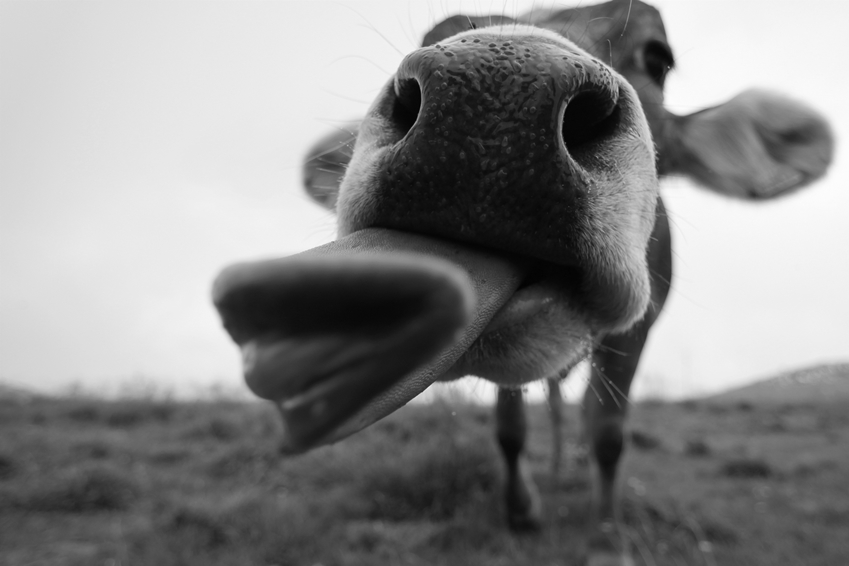
\includegraphics[width=0.9\textwidth]{03_GraphicFiles/CowLickingNose.jpg}
\captionsource{A cow licking its nose. Usage with permission of the photographer \textsc{Nicole Barth}}{Obtenido de \url{www.flickr.com/photos/46311827@N07/14885545396}, (2017)}
\label{fig:CowLickingNose}
\end{figure}

En la \figurename~\ref{fig:CowLickingNose}\myMarginnote{Reference to a figure} you see a cow that is licking its nose. The picture was taken by Nicole Barth on 11.08.2014 using a Canon EOS 500D. The original file has a resolution of $4247 \times 2831$ pixels\footnote{hola como te va}.


\begin{figure}[htb]
\centering
\begin{tikzpicture}
\begin{axis}[
axis lines = middle,
enlargelimits = true,
xlabel = {$x$},
ylabel = {$y$},
trig format plots = rad,
width = 0.9\textwidth,
height= 80mm,
title style={font=\bfseries,align=center,text width=0.7\textwidth},
title = {Example Diagram with a Line Break in the Title (using the \texttt{text width} option in the \texttt{title style})},
]
\addplot[myColorMainA,domain=0:9, line width=1pt, smooth]
{0.2*x^2};
\addplot[myColorMainB,domain=0:9, line width=1pt, smooth]
{5*sin(x)};
\end{axis}
\end{tikzpicture}
\captionsource{A scientific diagram using the \texttt{pgfplots} package by \textsc{Christian Feuersaenger} using the same colors which are also used for the layout}{Elaboración propia, (2017)}
\label{fig:ScientificDiagram}
\end{figure}

\Blindtext[2][2]

\begin{table}[htb]
\centering
\captiontable{A small table created with the \texttt{booktabs} package (example taken from the package documentation).}{Elaboración propia, (2017)}

\begin{tabular}{@{}llr@{}} \toprule
\multicolumn{2}{c}{Item} \\ \cmidrule(r){1-2}
Animal & Description & Price (\$)\\ \midrule
Gnat & per gram & 13.65 \\
& each & 0.01 \\
Gnu & stuffed & 92.50 \\
Emu & stuffed & 33.33 \\
Armadillo & frozen & 8.99 \\ \bottomrule
\end{tabular}

\end{table}


\Blindtext[2][1]

\section{Example Section}

\Blindtext[3][2]

\blinditemize

\section{Another Example Section}

\Blindtext[3][1]

\blindenumerate

\subsection{Example Sub-Section}

\blindmathpaper

\begin{figure}[htb]
\centering
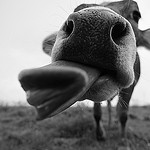
\includegraphics[]{03_GraphicFiles/CowLickingNoseSquare.jpg}
\captionsource{A cow licking its nose -- picture in square format in a native (low) resolution $150 \times 150$ pixels @ 72~dpi ($\approx 2.1$ inch). No scaling in \LaTeX{} using options in \texttt{\textbackslash includegraphics} is applied. Zoom in and see how ugly this is. See \figurename~\ref{fig:CowLickingNose} for reference.}{Elaboración propia, (2017)}
\label{fig:CowLickingNoseSquare}
\end{figure}

\subsection{Another Example Sub-Section}

\Blindtext[2][1]

\subsubsection*{Another Sub-Sub-Section}

\blindmathpaper

\paragraph{Example Paragraph}

\Blindtext[2][1]

\subparagraph{Example Sub-Paragraph}

\Blindtext[2][1]

\section{Yet Another Example Section}

\Blindtext[2][1]

% Final Thoughts
%%%% File encoding is UTF8
%%% You can use special characters just like ä,ü and ñ

\chapter{Final Thoughts}

\textquote[citation]{This is an incomplete sentence}.


%\Blindtext[2][1]

\printbibliography 
% Start appendix
\appendix

% Appendix A
%%% File encoding is UTF8
%%% You can use special characters just like ä,ü and ñ

\chapter{Capítulo Apéndice}



\section{Sección del apéndice}


\centering
\begin{neuralnetwork}[height=4]
	\newcommand{\nodetextclear}[2]{}
	\newcommand{\nodetextx}[2]{$x_#2$}
	\newcommand{\nodetexty}[2]{$y_#2$}
	\inputlayer[count=4, bias=false, title=Input\\layer, text=\nodetextx]
	\hiddenlayer[count=5, bias=false, title=Hidden\\layer, text=\nodetextclear] \linklayers
	\outputlayer[count=3, title=Output\\layer, text=\nodetexty] \linklayers
\end{neuralnetwork}

\begin{figure}[htb]
	\centering
	\begin{tikzpicture}
	\begin{axis}[axis lines = middle
	, enlargelimits = true
	, xlabel = {$x$}
	, ylabel = {$y$}
	, trig format plots = rad
	, width = 0.9\textwidth
	, height= 80mm
	, cycle list name=Dark2
	, title style={font=\bfseries,align=center,text width=0.7\textwidth}
	, title = {Example Diagram with a Line Break in the Title (using the \texttt{text width} option in the \texttt{title style})},
	]
	\addplot[myColorMainA,domain=0:9, line width=1pt, smooth]
	{0.2*x^2};
	\addplot[myColorMainB,domain=0:9, line width=1pt, smooth]
	{5*sin(x)};
	\end{axis}
	\end{tikzpicture}
	\captionsource{A scientific diagram using the \texttt{pgfplots} package by \textsc{Christian Feuersaenger} using the same colors which are also used for the layout}{\fuentePropia}
	\label{fig:ScientificDiagram}
\end{figure}

\subsection{Subseccion del apéndice}

% Appendix B
%%% File encoding is UTF8
%%% You can use special characters just like ä,ü and ñ

\chapter{Another Appendix Chapter}


%TODO: fix with cref
%Como se puede apreciar en la \cref{tab:b1}.
Como se puede apreciar en la \tab{tab:b1}.


\insertTableFile{Ejemplo de una tabla.}{Elaboración propia, (2017)}{04_Tables/CSVexample.csv}{\label{tab:b1}}

\end{document}
% ------------------------------------------------------------------
%
% #######################
% End: Document
% #######################
